\subsection{Implementación}

\begin{figure*}
\centering
	\includegraphics[width=0.9\textwidth]{../flowchart.jpg}
	\caption{Flow-chart del algoritmo.}
	\label{fig:Flowchart}
\end{figure*}

A partir de una selección del video proporcionada por el usuario se obtienen las mejores features del objeto seleccionado utilizando el algoritmo de Shi-Tomasi. Luego, mediante el algoritmo de Lucas-Kanade de Optical Flow se obtiene la evolución de las features en el tiempo. A este cúmulo de puntos se le calcula el centro de masas $\mu$ y el centro de inercia $\sigma$. Se rechazan los puntos de este cúmulo que se encuentren a una distancia mayor a $k_{\sigma}\sigma$ respecto al centro de masas, para luego calcular nuevamente el centro de masas el cual es el que se introduce en el filtro de Kalman como medición de la posición.

La dimensión del vector de estados del filtro de Kalman es de cuatro, poseyendo la posición y la velocidad tanto horizontal como vertical. La dimensión del vector de observación es de dos dado que solamente se mide la posición horizontal y vertical del centro de masas. La matriz $A$ queda definida por las ecuaciones que caracterizan el movimiento del objeto a seguir que, por simplicidad, se consideraron las ecuaciones cinemáticas de MRU, quedando entonces
\begin{equation}
\begin{pmatrix} x_{k-1} + dt\cdot v_{x_{k-1}} \\y_{k-1} + dt\cdot v_{y_{k-1}} \\ v_{x_{k-1}}  \\ v_{y_{k-1}} \end{pmatrix} =\begin{pmatrix}
1 & 0 & dt  & 0\\
0 & 1  & 0 & dt\\
0 & 0  & 1  & 0\\
0 & 0  & 0  & 1 
\end{pmatrix} \cdot \begin{pmatrix} x_{k-1}\\y_{k-1} \\ v_{x_{k-1}}  \\ v_{y_{k-1}} \end{pmatrix}
\end{equation}
Siendo, 
\begin{equation}
A = 
\begin{pmatrix}
1 & 0 & dt  & 0\\
0 & 1  & 0 & dt\\
0 & 0  & 1  & 0\\
0 & 0  & 0  & 1 
\end{pmatrix}
\end{equation}

Luego, se tiene que la matriz de observación o de transición de medición quedará definida por la transformación del espacio de observación al espacio real del vector de estados del filtro. Como los observables a medir forman parte del espacio real del vector de estados y son solo las posiciones, la matriz quedará definida de manera simple
\begin{equation}
\begin{pmatrix} z_{x_{k}} \\ z_{y_{k}} \end{pmatrix}=\begin{pmatrix}
1 & 0 & 0  & 0\\
%0 & 1  & 0 & 0  \end{pmatrix} \cdot  \begin{pmatrix} x_k \\ y_k \\ v_{x_{k}} \\ v_{y_{k}} \ver
\end{pmatrix}
\end{equation}
Siendo,
\begin{equation}
H = 
\begin{pmatrix}
1 & 0 & 0  & 0\\
0 & 1  & 0 & 0 
\end{pmatrix}
\end{equation}

Mientras que la matrices de covarianza del proceso $Q$ y de medición $R$ serán cuadradas por definición, de dimensión cuatro y dos respectivamente, y además de la forma $\mathbb{I}\cdot \xi$ dado que se asume independencia de las variables aleatorias, quedando

\begin{equation}
Q = 
\begin{pmatrix}
\xi_Q & 0 & 0  & 0\\
0 & \xi_Q  & 0 & 0\\
0 & 0  & \xi_Q  & 0\\
0 & 0  & 0  & \xi_Q 
\end{pmatrix}
\end{equation}

\begin{equation}
R = 
\begin{pmatrix}
\xi_R & 0 \\
0 & \xi_R 
\end{pmatrix}
\end{equation}

Siendo $\xi_Q$ y $\xi_R$ las varianzas del proceso y de medición respectivamente.

Finalmente, $\hat{x}_{k|k}$ y $P_{k|k}$ tomarán la forma

\begin{equation}
\hat{x}_{k|k} = 
\begin{pmatrix}
\hat{x}\\
\hat{y}\\
\hat{v_x}\\
\hat{v_y}
\end{pmatrix}
\end{equation}

\begin{equation}
P_{k|k} = 
\begin{pmatrix}
\gamma_{x} & 0 & 0  & 0\\
0 & \gamma_{y}  & 0 & 0\\
0 & 0  & \gamma_{v_x}  & 0\\
0 & 0  & 0  & \gamma_{v_y} 
\end{pmatrix}
\end{equation}

Siendo $\gamma_{i}$ la varianza de cada variable de estado. Cabe notar que el modelo utilizado asume independencia entre las variables aleatorias por simplicidad.
Este algoritmo, hasta ahora explicado, cuenta con grandes problemas. Dados dos objetos $A$ y $B$, donde $A$ es el objeto a seguir:

\begin{itemize}
\item Como el algoritmo de Shi-Tomasi tiende a colocar features en bordes bien definidos, y estos suelen ser los bordes externos de un objeto, si el objeto a seguir $A$ pasa por delante de un objeto $B$ con bordes bien definidos, las features del algoritmo de Optical Flow tenderán a adosarse a los bordes del objeto $B$ por más que este esté quieto.
\item Si el objeto $A$ pasase por detrás del objeto $B$ inmóvil, todas las features sobre el objeto a seguir quedarían adosadas al objeto $B$. Esto plantea un problema mucho más grande que el anterior, dado que no se podrá utilizar la estimación del filtro de Kalman de manera confiable, debido a que cuando los features se queden quietos adosados en $B$, se seguirá midiendo de todas formas y se seguirán entregando esas mediciones al filtro de Kalman, por lo que la estimación de este se adosará también al objeto $B$.
\item Profundizando en el item anterior, existe una ambigüedad entre que $A$ pase de un movimiento MRU a que se quede completamente quieto y que $A$ pase por detras de $B$, dado que en ambas situaciones las features quedarán quietas en el lugar donde $A$ se haya quedado quieto o el lugar de la intersección entre $A$ y $B$
\end{itemize}

La mejora propuesta para sortear este problema consiste en agregar un filtro de color, para diferenciar a $A$ y a $B$ por su color. La implementación de este filtro de color comienza en el momento que el usuario selecciona el área a seguir. Se calcula la mediana del color de la zona elegida, y ese color es transformado de formato RGB a formato HSV, o Hue-Saturation-Value, dado que es más sencillo definir una máscara de este modo. Dado $x$ e $y$ las coordenadas de los píxeles de la imagen, $\vec{R_k}$, $\vec{G_k}$ y $\vec{B_k}$ los vectores de píxeles de la selección, $mediana(\vec{R_k}, \vec{G_k}, \vec{B_k}) = (m_R, m_G, m_B)$ el vector que define la mediana del color de la selección, $\mathbb{HSV}$ el operador de transformación del espacio de coordenadas RGB a HSV, y $\mathbb{HSV}(m_R, m_G, m_B) = (m_H, m_S, m_V)$ el vector de la mediana del color de la selección en el espacio HSV, queda entonces definida la máscara de color como

\begin{equation}
f(x, y) = (f_h(x, y), f_s(x, y), f_v(x, y))
\end{equation}

\begin{equation}
f_{u}(x,y) = \left\{
\begin{array}{ll}


      1 & -\Lambda_u < u_{x, y} - m_u < \Lambda_u \\
      
      
      
      0 & \text{sino} \\
      
      
\end{array} 
\right.
\end{equation}

donde $\Lambda$ es el límite para cada propiedad $u$, siendo estas Hue, Saturation o Value. Una vez obtenida la máscara $f(x, y)$ se realiza una operación AND bit-a-bit entre la máscara y la imagen original, logrando obtener una intensidad nula en los píxeles de la imagen que no posean un color cercano a la mediana calculada como se puede ver en las Figuras (\ref{fig:col1}) y (\ref{fig:col2}).

\begin{figure}[H]
\centering
	\begin{subfigure}{.4\textwidth}
		\centering
		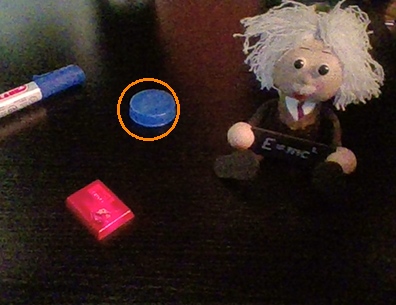
\includegraphics[width=\textwidth]{Imagenes/color1.png}
		\caption{Video antes de aplicar la máscara siguiendo al objeto azul.}
		\label{fig:col1}
	\end{subfigure}
	\begin{subfigure}{.4\textwidth}
		\centering
		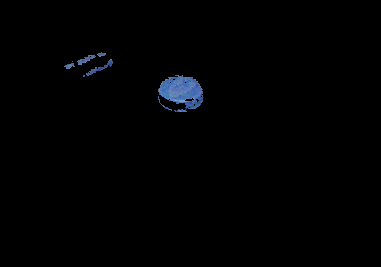
\includegraphics[width=\textwidth]{Imagenes/color2.png}
		\caption{Video después de aplicar la máscara. Es con esta imagen que opera el algoritmo y no con la normal.}
		\label{fig:col2}
	\end{subfigure}
	\caption{Comparación entre video normal y luego de aplicar la máscara.}
	\label{fig:color_comp}
\end{figure}

Este filtrado de color no solo posee una gran sinergia con el método de obtención de features de Shi-Tomasi, dado que este frame tendrá bordes de mucha mejor calidad, sino que tambíen posee una gran sinergia con el método de Optical Flow, debido a que como se verán menos bordes en la imagen modificada, aumenta notablemente la probabilidad de que los features queden contenidos todos dentro, o sobre los bordes del objeto a seguir.

Volviendo al caso de los objetos $A$ y $B$:

\begin{itemize}
\item Si $A$ y $B$ son de colores distintos, con el filtro de color, el algoritmo nunca detectará que existe un objeto $B$ por lo que seguirlo será imposible, y por consecuencia seguirá únicamente a $A$ y no se tendrá el problema de $A$ pasando por frente de $B$.
\item Si $A$ y $B$ son de colores distintos, y $A$, el objeto a seguir, pasa por detrás de $B$, ahora no se adosarán las features al objeto $B$, sino que el algoritmo verá que el área de $A$ se achica a medida que este queda oculto por $B$. Como los features no tendrán bordes para seguir, estos desaparecerán, por lo que se dejará de entregar mediciones al filtro de Kalman y este estimará correctamente la posición de $A$ mientras que este no haya sufrido aceleración alguna mientras estaba oculto. 
\end{itemize}

\begin{figure}[H]
\centering
	\begin{subfigure}{.4\textwidth}
		\centering
		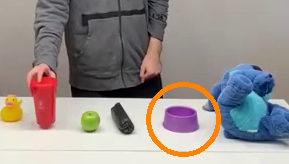
\includegraphics[width=\textwidth]{Imagenes/Optical1.png}
		\caption{Ventana con el funcionamiento normal del seguidor, el cual utiliza un círculo naranja para detallar donde se encuentra el objeto a seguir.}
		\label{fig:optical1}
	\end{subfigure}
	\begin{subfigure}{.4\textwidth}
		\centering
		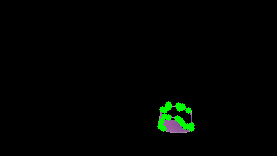
\includegraphics[width=\textwidth]{Imagenes/Optical2.png}
		\caption{Ventana la cual solo aparece al seleccionar el modo debug. Aquí se muestra si el filtro de color se encuentra activado, el video luego de pasar por la máscara de color, las features del objeto como puntos verdes y la zona de búsqueda si se diese el caso de tracking failure.}
		\label{fig:optical2}
	\end{subfigure}
	\caption{Resultado de la selección de un elemento.}
	\label{fig:optical12}
\end{figure}

Sin embargo, el filtro de Kalman no puede estimar la posición del objeto indefinidamente. Es por esto que cuando el objeto se pierde, es decir, no se logran detectar más features, se entra en otra fase del programa. En esta fase, se realiza una búsqueda del objeto en cada frame del video a partir de la estimación del filtro de Kalman y el tamaño original del área seleccionada. La altura y el ancho del área de búsqueda se incrementará por un factor constante por cada frame en la que la búsqueda falle. Esta búsqueda se basa en aplicar el algoritmo de Shi-Tomasi sobre el área mencionada.


Finalmente, para reforzar el algoritmo de seguimiento, se implemento además una recalculación periódica de las features con el método de Shi-Tomasi, partiendo de la media del cúmulo de features, removiendo los outliers, volviendo a calcular nuevamente la media y utilizar esta posición para aplicar el algoritmo de Shi-Tomasi, de misma manera que se realiza sobre la primera selección proporcionada por el usuario.

\subsection{Algoritmo correlación}
Para el algoritmo de correlacion no solo se utiliza el filtro explicado en la sección \ref{sec:corr} se realiza un filtrado de tanto el frame como el kernel, haciendo un cambio a \textbf{HSV} y un filtrado del frame en este espacio bajo las siguientes especificaciones: 
            
\begin{align}
MSK = H \  \epsilon \ (0,180 ) \ \ S \  \epsilon \ (50,255) \ \ V \ \epsilon \ (32,255)
\end{align}
luego se utiliza el filtro de correlación y se obtiene el punto donde esta es mayor, y se compara con el frame filtrado, si no comparte las características de color que son calculadas por el filtrado de color, este punto de correlación es desechado. Esto se logra aplicando una mascara en la sección de mayor correlación y sobre este realizar nuevamente el cálculo de máxima correlación. Se realizan unas pocas iteraciones con el propósito de no comprometer la velocidad de procesamiento entre frames. En caso de no encontrar al objeto se considera que hubo un error de trackeo (Oclusión del objeto).


\subsection{Optimización del Código}
Se realizó una optimización del codigo, quitando redundancias y utilizando únicamente librerías que son corridas en C++, se optó por un enfoque OOP. Esto permitió escalar el proyecto y una mayor modularidad. Contando con una GUI y la posibilidad de un trackeo multi-objeto, adicionalmente se puede interactivamente cambiar especificaciones de los trackers, al igual que diseñar el filtro de color para obtener el mejor resultado posible.


\subsection{KTN}

Se decidió implementar código en \textbf{Python}, apoyándose en la librería \href{https://opencv.org/}{OpenCV}.
El pseudocódigo que corresponde es:


\definecolor{keywords}{RGB}{255,0,90}
\definecolor{comments}{RGB}{0,0,113}
\definecolor{red}{RGB}{160,0,0}
\definecolor{green}{RGB}{0,150,0}
 
\lstset{language=Python, 
        basicstyle=\ttfamily\small, 
        keywordstyle=\color{keywords},
        commentstyle=\color{comments},
        stringstyle=\color{red},
        showstringspaces=false,
        identifierstyle=\color{green},
        procnamekeys={def,class}}
\begin{figure}[H]

\begin{lstlisting}
kalman = KalmanFilter()

cap = VideoCapture()

lower_thr, upper_thr = [],[]

prev = captureROI(cap)

prev = space_translate(x, y, prev)

frame = cap.read()

while(cap.isOpened()):

    frame_num++
    frame_real = cap.read()


    hsv = cvtColor(frame, COLOR_BGR2HSV)
    mask = inRange(hsv, lower_thr, upper_thr)
    frame = bitwise_and(frame, mask)

    if(recalc and not error):
        frame_num = 0
        prev, x, y = recalculateFeatures()

    if error:
        prev=  searchObject(kalman)
        dyn_h, dyn_w = new_dyn_h, new_dyn_w


    good_new, good_old,prev= measureFeatures()

    drawEstimate(good_new, kalman, frame)

\end{lstlisting}
\end{figure} 
 
 Finalmente se presenta un diagrama en bloques del programa, donde se puede apreciar como interaccionan todos los algoritmos trabajando en armonía.
\begin{figure}[H]
\centering
	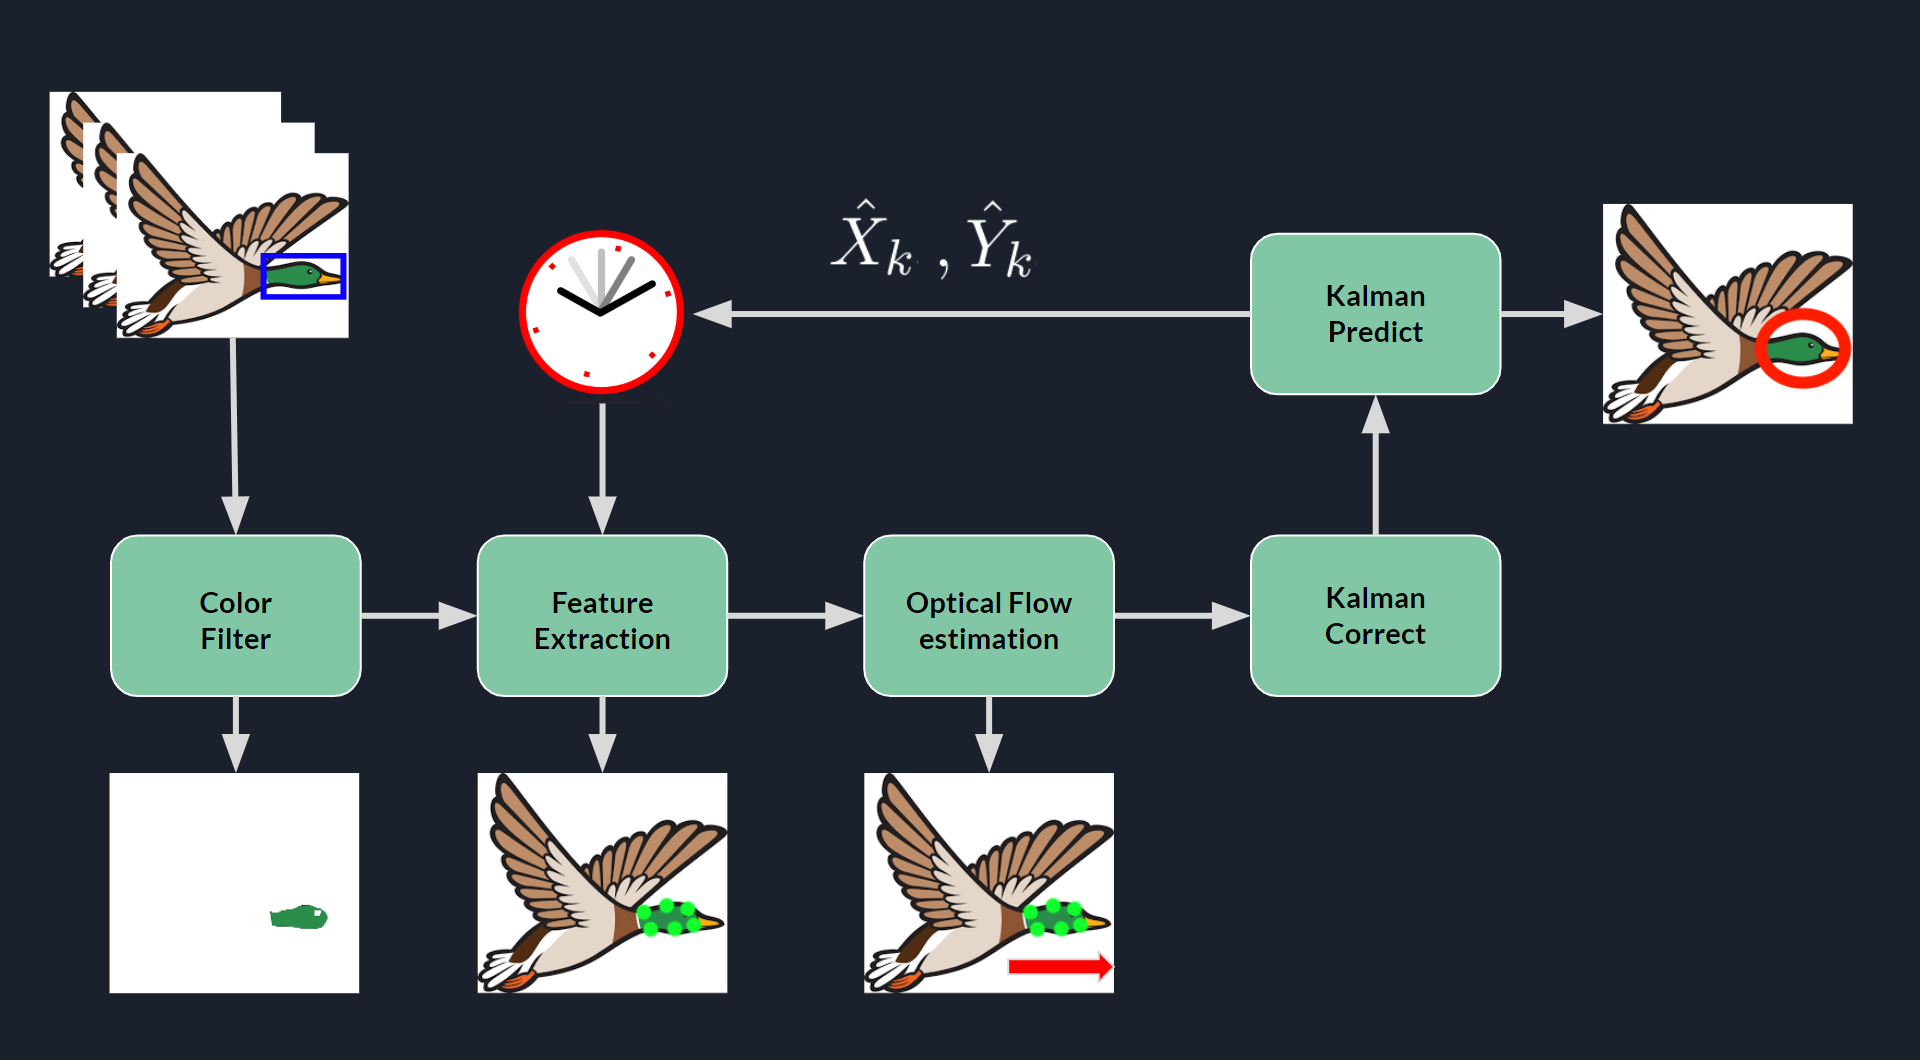
\includegraphics[width=0.5\textwidth]{Imagenes/diagram.png}
	\caption{Diagrama en bloques del programa.}
	\label{fig:bloques}
\end{figure}


\subsection{Escenarios de fallas}
Algunos casos donde puede fallar el Tracker son:
\begin{itemize}
\item El cambio de trayectoria de un objeto una vez que desaparece, provocará una falla en la predicción.
\item Interacción entre el objeto trackeado y un objeto de características similares, puede causar un error de detección
\item Cambios bruscos de iluminación o en color del objeto.

\end{itemize}

